\section{Simulation}
\label{sec:Chapter2} \index{Chapter2}


Для задач квантового машинного обучения разработаны ряд фреймворков \cite{bergholm2018pennylane}. Стандартные подходы к оптимизации параметров квантовых систем опираются на эволюцию с использованием параметризованных квантовых гейтов. Такая динамика легко поддаётся симуляции, поскольку сводится к вычислению матричных экспонент от постоянных гамильтонианов. В свою очередь, симуляция эволюции системы ридберговских атомов представляет собой значительно более сложную вычислительную задачу.

Как отмечалось в разделе \ref{seq:qnn_intro}, зависимость гамильтонина от времени не позволяет получить оператор эволюции аналитическим способом. В связи с этим, его нахождение требует ресурсоёмких численных методов вычисления Т-экспоненты. Такой подход реализован в библиотеках PennyLane и Bloqade \cite{bergholm2018pennylane,bloqade2024sdk}. Следовательно симуляция эволюции даже с одним набором параметров занимает значительное время, что делает непрактичным обучение QML моделей, требующих многократных итераций. Для преодоления этого ограничения нами был разработан симулятор для эффективного расчёта динамики ридберговских систем.

Основынми целями были максимальное ускорение вычислений и реализация параллельной симуляции систем с разными параметрами, что необходимо для batch processing. Поэтому в качестве основного фрейморка был выбран JAX \cite{bradbury2018jax}, который ускоряет вычисления за счёт JIT-компиляции и предоставляет нативные средства для векторизации операций.



Ключевой проблемой является вычисление Т-экспоненты, решение которой требует упрощения системы. Мы отказались от поддержки произвольных временных зависимостей функций $\Omega(t)$, $\varphi(t)$ и $\delta(t)$, ограничившись их кусочно-постоянной параметризацией, описанной в разделе \ref{seq:qnn_intro}. Однако даже при таких условиях эволюция не вычисляется аналитически из-за линейных переходов между сегментами. 

Чтобы свести симуляцию к произведению экспонент от постоянных гамильтонианов, мы аппроксимировали каждый линейный переход равномерно конечным числом кучосно-постоянных шагов. Пример такой аппроксимации представлен на Рисунке \ref{fig:steps_approximation}.  Очевидно, что такой подход вносит контролируемую погрешность в симуляцию, но позволяет кардинально ускорить вычисления, за счёт аналитического рассчёта оператора эволюции. Точность аппроксимации увеличивается с числом шагов, как изображено на Рисунке \ref{fig:errors_comparison} (слева).

\begin{figure}[h!] \label{fig:steps_approximation}
    \centering
    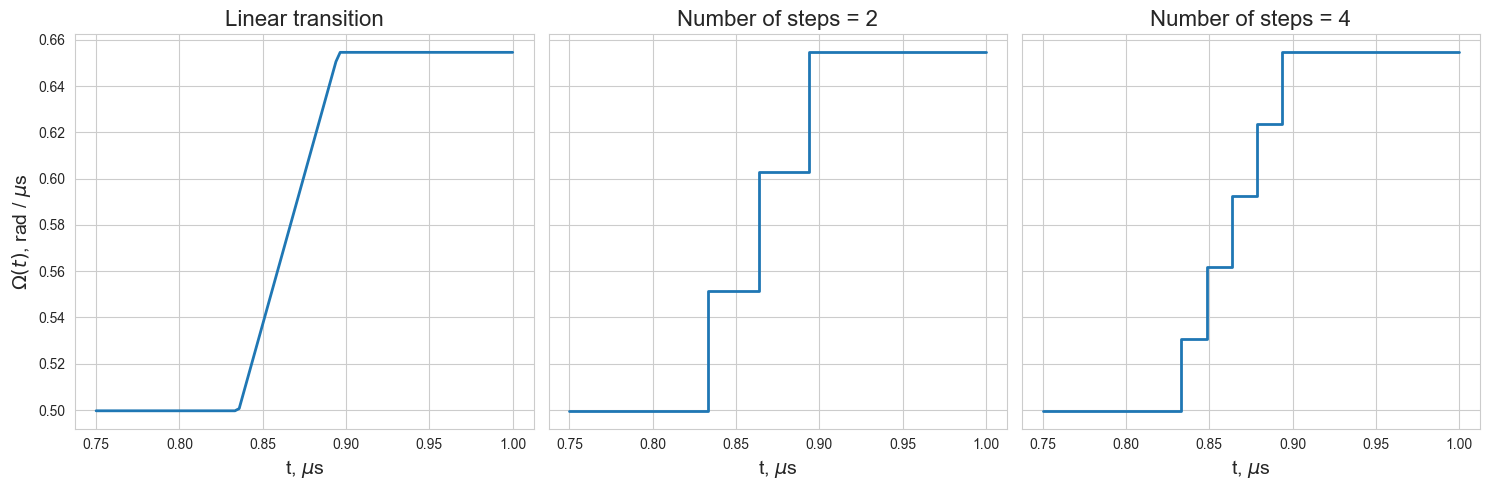
\includegraphics[width=1\linewidth]{images/steps_plot.png}
    \caption{Пример кусочно-постоянной равномерной аппроксимации одного линейного перехода частоты Раби с использованием двух и четырёх шагов.}
\end{figure}



При работе с реальным квантовым компьютером невозможно измерить конечную волновую функцию. Поэтому средние значения наблюдаемых величин оцениваются посредством многократных проективных измерений, что вносит стастическую ошибку, известную как shot noise. Этот аспект даёт конструктивный физический критерий для выбора числа шагов аппроксимации: нужно увеличивать шаги до тех пор, пока ошибка симуляции не станет сопоставимой с shot noise. Фреймворк bloqade, совместимый с квантовым компьютером Aquila, предоставляет возможность проводить симуляцию его работы с учётом shot noise. На Рисунке \ref{fig:errors_comparison} (справа) представлена зависимость относительная ошибки, вызванной shot noise, от числа шотов. На практике обычно используется $10^3 \sim 10^4$ шотов. Сравнение двух графиков показывает, что использование всего 2 шагов аппроксимации вносит ошибку меньше shot noise в рабочем диапазоне.

\begin{figure}[h!] \label{fig:errors_comparison}
    \centering
    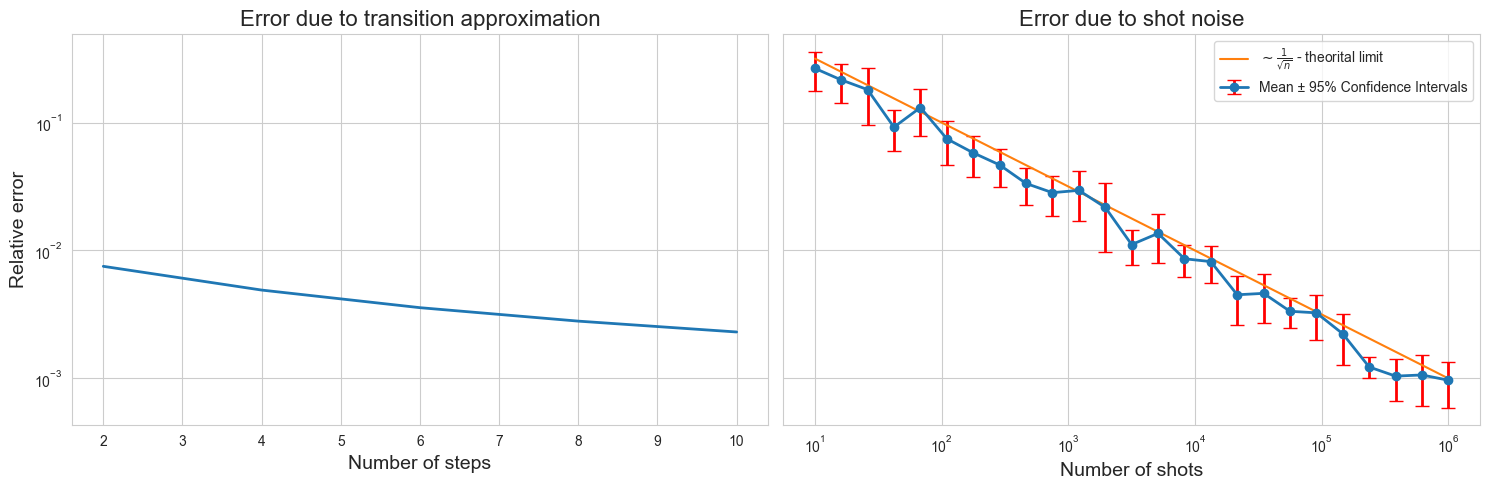
\includegraphics[width=1\linewidth]{images/errors_plot.png}
    \caption{Сравнение источников ошибки в log-log масштабе. \textbf{Слева:} Зависимость относительной ошибки симуляции от числа шагов аппроксимации. \textbf{Справа:} Зависимость относительной ошибки от числа измерений. Доверительный интервалы построены по результатам 10 экспериментов. Оранжевая кривая соответствует теоретическому пределу $1 / \sqrt{n}$, следующему из центральной предельной теоремы.}
\end{figure}

\subsection{Rydberg Blockade} \label{seq:bloqade}
Одной из ключевых особенностей ридберговских систем является сильное взаимодействие Ван-дер-Ваальса. Как показано в уравнении \ref{eqn:van_der_waals_interaction}, энергия этого взаимодействия $V_{ij} \propto C_6/r_{ij}^6$ убывает с расстоянием $r_{ij}$ и характеризуется аномально большим коэффициентом $C_6$. Поэтому, когда атомы расположены достаточно близко, энергия их взаимодействия может значительно превышать частоту Раби. В этом режиме, известном как \textbf{Ридберговская блокада}, одновременное возбуждение обоих атомов оказывается подавленным.

Эта особенность крайне полезна для симуляции квантовой динамики, поскольку позволяет значительно снизить вычислительные ресурсы. Достигается это с помощью проецирования на эффективное подпространство, из которого исключены запрещённые состояния. Чтобы качественно оценить вклад от этого эффекта, рассмотрим систему из $n$ атомов, расположенных в одномерную цепочку на одинаковом расстоянии друг от друга. Введем параметр <<радиус блокады>> $R_b$, определяющий расстояние, в пределах которого одновременное возбуждение двух атомов запрещено. Будем считать, что этот радиус охватывает $k$ атомов.

Положим $p_n$ ранвым размерности гильбертова пространства разрешённых состояний. В терминах битовых строк $p_n$ равно количеству строк длины $n$, в которых в любом окне длины $k$ содержится не более одной единицы. Легко получить рекурентную формулу для $p_n$, рассмотрев 1-й элемент битовой строки:
\begin{itemize}
    \item Если 1-й элемент равен 0, то он не влияет на ограничения для следующих $n-1$. Значит число таких строк равно $p_{n-1}$.
    \item Если 1-й элемент равен 1, то в силу блокады все следующие за ним $k-1$ биты должны быть нулями. На оставшиеся $n-k$ атомов накладываются исходные ограничения, и число таких конфигураций равно $p_{n-k}$.
\end{itemize}
Суммируя эти два случая, приходим к рекурентному соотношению:
\begin{equation}
    p_n = p_{n-1} + p_{n-k}.
    \label{eqn:blockade_recurrence}
\end{equation}
В качестве граничных условий можно положить $p_n = n+1$ для $1 \le n \le k$, поскольку радиус блокады охватывает всю систему.

Решение данного линейного рекурентного уравнения определяется характеристическими числами, удовлетворяющими уравнению:
\begin{equation}
    x^{k} = x^{k - 1} + 1.
\end{equation}
Оно всегда имеет доминирующий корень $\lambda_k \in (1, 2)$, который определяет асимптотику $p_n \sim c \cdot \lambda_k^n$ \cite{ConcreteMath}. Значит при фиксированном $k$ размерность эффективного гильбертова пространства всё ещё растёт экспоненциально, но с показателем значительно меньшим 2. Зависимость размерности подпространства от параметра $k$ для системы из 10 атомов показана на Рисунке \ref{fig:blockade_analysis} (слева).

\begin{figure}[h!]
    \centering
    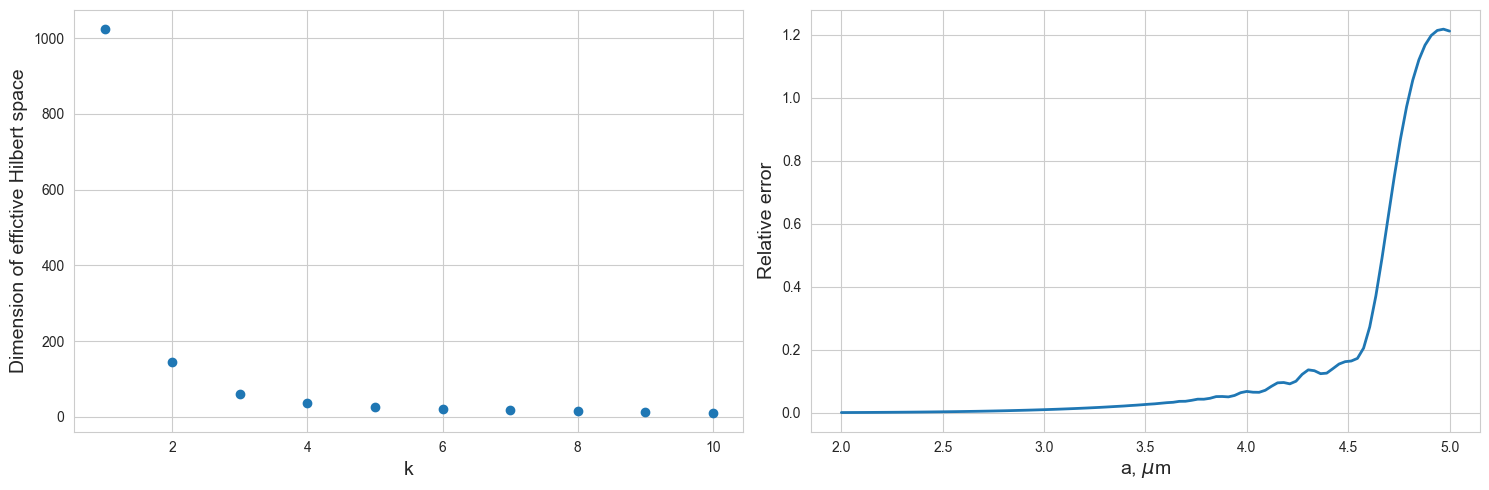
\includegraphics[width=1\linewidth]{images/bloqade_plot.png}
    \caption{Графический анализ ридберговской блокады. \textbf{Слева:} Зависимость размерности гильбертова пространства разрешённых состояний от числа заблокированных атомов $k$ для цепочки из 10 атомов. Размерность полного пространства $2^{10}=1024$. \textbf{Справа:} Зависимость относительной ошибки аппроксимации ридберговской блокады от расстояния между атомами для системы из 3 атомов. Эффективный радиус блокады $R_b$ соответствует началу экспоненциального роста ошибки и в данном случае равен $4.5 \mu m$.}
    \label{fig:blockade_analysis}
\end{figure}

Остается вопрос об определении радиуса блокады $R_b$, поскольку блокада является аппроксимацией к настоящей эволюции в полном пространстве. Точность этой аппроксимации определяется отношением величины межатомного взаимодейтсвия к параметрам лазерного воздействия. Для численного определения $R_b$ можно использовать следующий подход:
\begin{enumerate}
    \item Радиус блокады полагается условно бесконечным, при котором все атомы заблокированы.
    \item Проводится симуляция с учётом блокады. 
    \item Проводится серия экспериментов с разным расстоянием между атомами без блокады.
    \item Для каждого эксперимента вычисляется ошибка симуляции как относительная норма разности конечных волновых функций.
\end{enumerate}
На графике зависимости ошибки симуляции от расстояния $a$ будет наблюдаться следующее поведение: при малых $a$ ошибка мала, но по мере увеличения расстояния начинается экспоненциальный рост. Точка, соответствующая переходному моменту принимается за эффективный радиус блокады $R_b$. Пример такого графика показан на Рисунке \ref{fig:blockade_analysis} (справа).
